\scanpage{35}
\mspage{2}
\textcircled{4} \(\nu=2\). \deleted{Il y a \unsure{deux cas}} \inserted{\unsure{Dans ce cas|Dans les}} \(K^g=\{P\}\), et \(K\setminus K^g\) \inserted{\(=I\)} est réunion de deux orbites. Ainsi, \(g\) est un autom. \deleted{\unsure{de}} ``universel'' de \(\Sigma\setminus I\) (\(g\in V(\unsure{D_I|\mathbb D_I})\)) et \(P\) est \inserted{\unsure{un de|un|un aut.}} \unsure{\deleted{un}|un} p\textsuperscript{t} fixe. \deleted{\unsure{De|Ce}} Cette fois, la situation \unsure{a} des ``modules'', p.ex. en choisissant une des deux orbites,

\deleted{\unsure{OPS} \unsure{que|pour} l’opération de \(\unsure{g|\langle g\rangle}\) sur elle est celle de \(\mu_2\) \inserted{\(=\{\pm1\}\)} sur \(\mu_2\) \inserted{\(=\unsure{\{\pm1\}|(\pm1)}\)}, et \(P=0\), l’autre orbite est \deleted{\unsure{donnée par}} \unsure{un|une} \(\{t,-t\}\), avec \(\lambda=t^2\ne1,\lambda\in k^\times\) ---
donc \deleted{\(\lambda=\)} \(J=(0,\pm1,\pm\unsure{\sqrt\lambda|t})\) \deleted{\(\unsure{\sqrt\lambda,\sqrt\lambda)|\sqrt\lambda,-\sqrt\lambda)}\)}, avec \(\lambda\in\Sigma(k)\setminus\{0,1,\infty\}\),
\unsure{Si on|en} \deleted{\unsure{change}} change le choix de l’orbite, on trouve
\[
(0,\pm1,\pm\sqrt{1/\lambda}).
\]
Prenons le paramètre \(\rho=\lambda+\frac1\lambda\), \inserted{\(\ne2\)}, donc \(\lambda^2-\rho\lambda+1=0\);
\deleted{\(\lambda=\frac12(\rho\pm\sqrt{\rho^2-4})\)},
on trouve \((0,\pm1,\pm\sqrt{\frac12(\rho\pm\sqrt{\rho^2\unsure{-4}})})\).
\unsure{Eliminer|Comme} \(0,\infty\), et \unsure{deux|les} \unsure{discriminant} \(\lambda\longrightarrow1\), ou --- \unsure{comme} \deleted{\(\unsure{f^\circ|\rho}\)} \(\lambda\), et
\(g(z)=\frac{\lambda}{z}\), p\textsuperscript{ts} fixes}

Cas moins intéressant que les précédents, \unsure{du|de} notre point de vue, car il y a des modules. Quand la structure \((\Sigma,I)\) est une structure carrée, on retrouve soit le cas \(2^\circ\) (si \(g\) laisse stables les deux diagonales), soit le cas \inserted{des sommets} d’un \deleted{\unsure{carré|cas|cube}} carré sphérique équilatéral, et du milieu de l’une des arêtes. \inserted{Est-ce le cas \(1^\circ\) ?} Quand c’est une structure tétraédrale, \(P\) est un des \inserted{\(6\)} sommets de l’octaèdre associé.

\figure{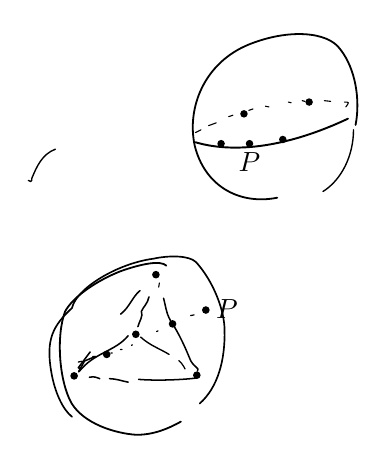
\begin{tikzpicture}[x=.0088cm,y=-.0088cm,line cap=round,line join=round]
% Upper sphere: the contour is open at lower right and has a short right-side gap.
\draw[line width=.65pt] (383,249)
 .. controls (327,260) and (278,231) .. (264,174)
 .. controls (252,119) and (278,54) .. (342,28)
 .. controls (399,5) and (456,9) .. (474,35)
 .. controls (496,63) and (503,108) .. (496,144);
\draw[line width=.5pt] (493,151)
 .. controls (493,188) and (476,223) .. (449,240);
\draw[line width=.7pt] (265,169)
 .. controls (323,186) and (400,175) .. (485,135);
% Rear equatorial arc, with the irregular short dashes visible on the sheet.
\draw[line width=.4pt] (265,155)--(273,151)
 (284,145)--(295,141) (313,132)--(319,130)
 (342,123)--(348,121) (366,117)--(371,118)
 (399,111)--(403,112) (419,109)--(423,110)
 (451,109)--(460,110) (480,111)..controls(487,111)..(482,118);
\foreach \x/\y in {302/171,343/171,391/165,335/128,429/111}
 {\fill (\x,\y) circle[radius=5.4];}
\node[below,inner sep=1pt] at (343,179) {$P$};
% Detached curved stroke at the left, without a supplied arrowhead.
\draw[line width=.5pt] (63,179)..controls(44,186)and(36,204)..(29,221)
 ..controls(30,227)and(25,226)..(24,224);
\begin{scope}[shift={(25,305)}]
% Lower sphere: the two left-hand contours and the open lower-right contour.
\draw[line width=.65pt] (198,42)
 ..controls(190,34)and(163,39)..(132,50)
 ..controls(99,63)and(64,86)..(52,108)
 ..controls(39,143)and(43,207)..(61,240)
 ..controls(79,270)and(124,284)..(155,286)
 ..controls(180,286)and(201,277)..(219,267);
\draw[line width=.6pt] (62,103)
 ..controls(34,129)and(24,149)..(32,195)
 ..controls(37,225)and(49,250)..(62,260);
\draw[line width=.6pt] (62,103)
 ..controls(68,75)and(127,39)..(179,32)
 ..controls(202,27)and(231,27)..(241,37)
 ..controls(267,66)and(282,108)..(282,135)
 ..controls(283,179)and(272,218)..(246,241);
% Broken outer triangular sides and rear branches, preserving their gaps.
\draw[line width=.55pt] (160,78)..controls(149,87)and(145,102)..(132,112);
\draw[line width=.55pt] (88.1778,166.4)--(71.1111,189.1556)--(74.6667,191.6444);
\draw[line width=.55pt] (71.4667,194.8444)--(80,179.5556)--(95.2889,173.1556);
\draw[line width=.55pt] (194,89)..controls(198,104)and(198,113)..(207,126)
 ..controls(216,140)and(224,157)..(231,174)
 ..controls(236,189)and(247,189)..(243,194);
\draw[line width=.55pt] (87,203)..controls(94,201)and(99,204)..(102,205)
 (116,205)..controls(126,205)and(136,209)..(143,210)
 (158,206)..controls(180,208)and(219,207)..(242,204);
\draw[line width=.55pt] (173,87)..controls(171,97)and(165,101)..(162,108)
 ..controls(165,115)and(159,122)..(157,130);
\draw[line width=.55pt] (143,143)..controls(124,166)and(94,167)..(72,195);
\draw[line width=.5pt] (161,145)..controls(174,157)and(189,162)..(202,170);
\draw[line width=.45pt] (216,179)..controls(220,182)and(223,187)..(225,191);
% Dotted oblique slant, including the short dash next to P.
\draw[line width=.45pt] (71,181)--(76,180) (92,173)--(97,173)
 (118,168)--(120,168) (132,163)--(134,163)
 (148,157)--(149,156) (184,137)--(186,136)
 (233,114)--(238,113);
\draw[line width=.4pt] (188,67)--(187,73);
\foreach \x/\y in {183/55,65/201,242/200,154/141,112/170,207/126,255/106}
 {\fill (\x,\y) circle[radius=5.5];}
\node[right,inner sep=2pt] at (261,105) {$P$};
\end{scope}
\end{tikzpicture}}

\uline{Cas des antiautomorphismes \inserted{\(\sigma\)} de} \(\Sigma\) laissant \uline{stables} \(K\). \inserted{\unsure{(}Cas \(k=\mathbb C\))} Comme \unsure{il|\(\sigma\)} est d’ordre pair, on voit qu’il \deleted{\unsure{et|a}} \unsure{a|.} un p\textsuperscript{t} fixe au moins dans \(K\), donc dans \(\Sigma\), et étant d’ordre fini, on sait qu’il est d’ordre \(2\), il correspond à une structure réelle sur \(\Sigma\), \deleted{\unsure{et}}
On distingue suivant le cardinal de \(K^\sigma\), qui est \(1,3\), ou \(\unsure{6|5}\).
\margin{34}
